\section{ownCloud installieren}

\subsection{Abhänigkeiten installieren}
Damit ownCloud reibungslos laufen kann, müssen einige zusätzliche Pakete installiert werden.
\\
Folgende Hauptkomponenten werden benötigt:

\begin{itemize}
\item Apache2 \\
Apache2 ist ein freier Webserver. Als Webserver wird ein Dienst bezeichnet, der Anfragen über das Web empfangen und beantworten kann. Ein Webbrowser - beispielsweise Mozilla Firefox - ist das Gegenstück zum Webserver. Er ist derjenige, der die Anfragen an den Server sendet. In unserem Fall ist die Aufgabe von Apache2, das installierte ownCloud für einen Client erreichbar zu machen.
\item PHP5 \\
ownCloud wurde mit der Scriptsprache PHP programmiert. Die PHP-Komponente (PHP5) muss zusätzlich zu Apache installiert werden, damit ownCloud als Anwendung überhaupt ausgeführt werden kann.
\item SQLite \\
Um Benutzerdaten wie Benutzername und Passwort zu speichern, braucht es eine Datenbank. Diese stellt SQLite zur Verfügung.
\end{itemize}

Der folgenden Befehl kann entweder kopiert und ins Terminal eingefügt oder aber abgetippt werden. Je nach verwendetem PDF-Betrachter, muss auf die 2. Methode zurückgegriffen werden:

\begin{lstlisting}
sudo apt-get install apache2 php5 php5-gd php5-sqlite php5-curl php5-json php5-common php5-intl php-pear php-apc php-xml-parser libapache2-mod-php5 curl libcurl3 libcurl3-dev sqlite
\end{lstlisting}

\subsection{Statische IP-Adresse}
Die IP-Adresse, durch welche der Computer im Netz eindeutig identifiziert werden kann und über welche letztendlich der Zugriff auf die Cloud erfolgt, kann nach jedem Computerstart anders aussehen.
Aus diesem Grund ist es sinnvoll, die IP-Adresse statisch festzulegen.
\\
\\
Zuerst muss die Netwerkkonfigurationsdatei unter \textit{/etc/network/interfaces} angepasst werden. Dazu muss man die Datei mit einem Texteditor öffnen. In diesem Tutorial wird der vorinstallierte Texteditor \textit{nano} verwendet: 

\begin{lstlisting}
sudo nano /etc/network/interfaces
\end{lstlisting} 

\begin{figure}[H]
\centering
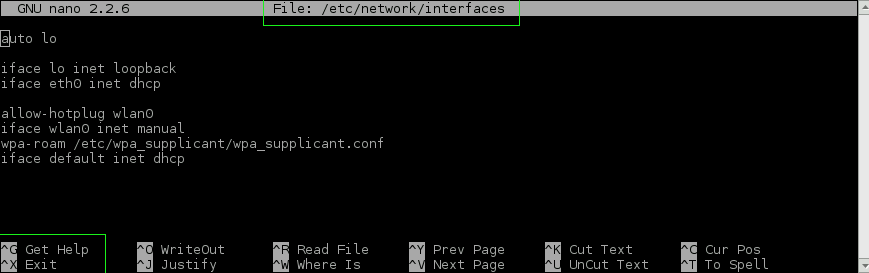
\includegraphics[scale=0.6]{images/nano}
\caption{Texteditor nano}
\end{figure}

Unter Umständen kann es vorkommen, dass folgende Zeile bereits in der Datei steht:

\begin{lstlisting}
iface eth0 inet dhcp
\end{lstlisting}

Wenn das der Fall ist, muss sie gelöscht und durch folgende Zeilen ersetzt werden:

\begin{lstlisting}
iface eth0 inet static
address 192.168.1.107
netmask 255.255.255.0
gateway 192.168.1.1
network 192.168.1.0
broadcast 192.168.1.255
\end{lstlisting}

Die verwendete IP-Adresse in der zweiten Zeile (192.168.1.107) sollte durch die aktuelle IP-Adresse des Systems ersetzt werden. Diese kann mit dem Kommando \textit{ifconfig} ermittelt werden.

\begin{figure}[H]
\centering
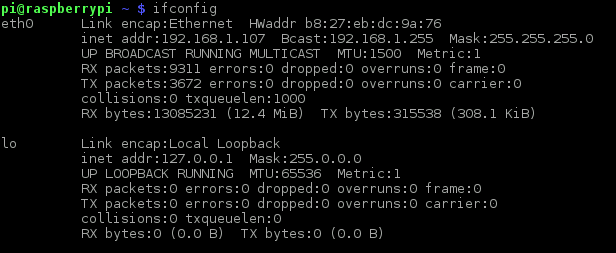
\includegraphics[scale=0.65]{images/ifconfig}
\caption{Ausgabe von ifconfig}
\end{figure}

Nun muss das Interface \textit{eth0} (Netzwerkschnittstelle) noch neu gestartet werden, damit die Änderungen wirksam werden:

\begin{lstlisting}
ifdown eth0
ifup eth0
\end{lstlisting}

\subsection{Webserver-Benutzer anlegen}
Aus Sicherheitsgründen sollte ein Webserver immer von einem Benutzer mit eingeschränkten Rechten betrieben werden. Er soll schliesslich nur auf jene Dateien zugreifen können, die er auch wirklich braucht. Dazu legt man einen Benutzer namens \textit{www-data} an und fügt ihn der gleichnamigen Gruppe zu:

\begin{lstlisting}
groupadd www-data
usermod -a -G www-data www-data
\end{lstlisting}

Nach dem Befehl \textit{groupadd} wird unter Umständen eine Meldung angezeigt, dass die angegebene Gruppe bereits existiert. Dies ist nicht weiter schlimm und man kann mit dem zweiten Befehl fortfahren.

\subsection{Webserver konfigurieren}
Als Webserver wird Apache2 verwendet, den man zuvor bereits installiert hat. Er muss jetzt lediglich noch so eingerichtet werden, dass ownCloud darauf ausgeführt werden kann.
\\
\\
Apache verlangt beim Start zu wissen, wie der Webserver heisst. Man hat hier freie Wahl, sollte aber etwas Sinnvolles wie beispielsweise \textit{owncloud} eingeben.
\\
Jetzt muss der Name der Konfigurationsdatei von Apache hinzgefügt werden:

\begin{lstlisting}
echo "ServerName owncloud" >> /etc/apache2/apache2.conf
\end{lstlisting}

Auch dem System selbst muss dieser Namen bekannt gegeben werden. Folgender Befehl fügt die entsprechende Zeile der Datei \textit{/etc/hosts} hinzu:

\begin{lstlisting}
echo "127.0.0.1 ownloud" >> /etc/hosts
\end{lstlisting}

Damit ownCloud überhaupt ausgeführt werden darf, müssen ihm noch gewisse Rechte eingeräumt werden. Dazu öffnet man die Apache Konfigurationsdatei \textit{/etc/apache2/sites-enabled/000-default} mit einem Texteditor:

\begin{lstlisting}
nano /etc/apache2/sites-enabled/000-default
\end{lstlisting}

Und sucht nach folgendem Abschnitt:

\begin{lstlisting}
<Directory /var/www/>
  Options Indexes FollowSymLinks MultiViews
  AllowOverride None
  Order allow,deny
  allow from all
</Directory>
\end{lstlisting}

Die Zeile \textit{AllowOverride None} einfach mit \textit{AllowOverride All} ersetzen. Zum Schluss müssen noch ein paar zusätzliche Module für den Webserver installiert werden:

\begin{lstlisting}
a2enmod rewrite
a2enmod headers
\end{lstlisting}

\subsection{Webserver absichern}
Ein grosses Thema in Sachen Cloud ist die Sicherheit. Die zukünftige Cloud soll dabei nicht zu kurz kommen, weshalb der Webserver mit HTTPS\footnote{\url{http://de.wikipedia.org/wiki/Https}}
ausgestattet wird.
\\
\\
Zuerst muss ein Zertifikat mit Schlüssel generiert werden. Anschliessend wird dieses in ein bestimmtes Verzeichnis abgelegt, damit der Webserver es auch finden kann.
\\
Folgende Befehle müssen dazu der Reihe nach abgesetzt werden:

\begin{lstlisting}
mkdir -p /etc/apache2/ssl

openssl req -new -x509 -days 365 -nodes -out /etc/apache2/ssl/apache.pem -keyout /etc/apache2/ssl/apache.pem

ln -sf /etc/apache2/ssl/apache.pem /etc/apache2/ssl/`/usr/bin/openssl x509 -noout -hash < /etc/apache2/ssl/apache.pem`

chmod 600 /etc/apache2/ssl/apache.pem
\end{lstlisting}

Nach der Erstellung des Zertifikates muss das Modul geladen werden, welches ownCloud mit SSL (HTTPS) ausstattet:

\begin{lstlisting}
a2enmod ssl
\end{lstlisting}

Nun muss das das Verzeichnis \textit{/var/www} noch mit SSL verknüpft werden. Dazu öffnet man folgende Datei mit einem Texteditor: 

\begin{lstlisting}
nano /etc/apache2/sites-available/ssl
\end{lstlisting}

Und fügt folgende Zeilen hinzu: 

\begin{lstlisting}
<virtualhost *:443>
  SSLEngine On
  SSLCertificateFile /etc/apache2/ssl/apache.pem
  DocumentRoot /var/www  
</virtualhost>" 
\end{lstlisting}

Anschliessend wird die vorgenommene Konfiguration noch aktiviert:

\begin{lstlisting}
a2ensite ssl
\end{lstlisting}

\subsection{PHP konfigurieren}
Die PHP-Komponente des Webservers muss ebenfalls angepasst werden. Sie hat standardmässig ein Sicherheitslimit gesetzt, welches die Uploadgrösse einer Datei einschränkt. Dieses soll nun aber erhöht werden, damit der Anwender der Cloud in der Lage ist, Dateien hochzuladen, die grösser als 2 bzw. 8 Megabyte sind. In diesem Beispiel wird das Limit auf 2GB (Gigabyte) gesetzt.
\\

\begin{lstlisting}
sed -i 's/upload_max_filesize = 2M/upload_max_filesize = 2G/' /etc/php5/apache2/php.ini

sed -i 's/post_max_size = 8M/post_max_size = 2G/' /etc/php5/apache2/php.ini
\end{lstlisting}

\subsection{ownCloud installieren}
Jetzt ist der Webserver bereit, um ownCloud zu installieren. Zuerst muss die neuste Version von ownCloud heruntergeladen werden. Um herauszufinden, welches die neuste Version ist, besucht man am besten die offizielle Webseite\footnote{\url{https://owncloud.org/}} oder Wikipedia. Zur Zeit ist Version 6.0.1 die Aktuellste. Sie kann wie folgt direkt aus der Konsole heruntergeladen werden:

\begin{lstlisting}
cd
wget http://download.owncloud.org/community/owncloud-6.0.1.tar.bz2 -O owncloud.tar.bz2
\end{lstlisting}

Nun muss das heruntergeladene Archiv noch entpackt und die Dateien in den Ordner \textit{/var/www} verschoben werden. Dieser Ordner ist standardmässig der vom Webserver benutzte.

\begin{lstlisting}
tar xvf owncloud.tar.bz2
rm -f /var/www/index.html
mv owncloud/* /var/www
mv owncloud/.htaccess /var/www
rm -rf owncloud owncloud.tar.bz2
\end{lstlisting}

Damit der zuvor erstellte Benutzer \textit{www-data} auch auf diese Dateien zugreifen kann, müssen ihm noch die entsprechenden Rechte gegeben werden:

\begin{lstlisting}
chown -R www-data:www-data /var/www
\end{lstlisting}

\subsection{Speicher erweitern}
Da die verwendete SD-Karte eine eher kleine Kapazität hat, lohnt es sich, ownCloud mehr Speicher zur Verfügung zu stellen. Man kann dazu eine externe Festplatte per USB bzw. einen USB-Stick an den Raspberry anschliessen und konfigurieren.
\\
\\
Zuerst muss man den Namen des angeschlossenen Speichergerätes herausfinden: 

\begin{lstlisting}
blkid
\end{lstlisting}

Dieser Befehl gibt alle angeschlossenen Speichergeräte an. Wenn neben der SD-Karte lediglich ein zusätzliche Speichergerät angeschlossen wurde, müsste dieses als drittes aufgeführt sein mit der Bezeichnung \textit{dev/sda1}.

\subsubsection{Separater Speicher}
Wird ein neues oder leeres Speichergerät verwendet, muss es zuerst neu formatiert werden (hier mit dem Dateisystem ext4).
\\Achtung: Dies löscht alle auf dem Speichergerät vorhandenen Daten!
\\
\begin{lstlisting}
mkfs.ext4 /dev/sda1
\end{lstlisting}

Dieser Schritt kann auch weggelassen werden. Es ist aber grundsätzlich empfohlen, für ownCloud ein separates Speichergerät zu verwenden.

\subsubsection{Automatisches Einbinden}
Damit die Festplatte bei jedem Neustart automatisch eingebunden (aktiviert) wird und zur Verfügung steht, muss das System dementsprechend konfiguriert werden. 
\\
\\
Zuerst wird das Verzeichnis erstellt, unter dem das Speichergerät später eingebunden wird:

\begin{lstlisting}
mkdir -p /mnt/ownclouddata
\end{lstlisting}

Dann muss der Typ des auf dem Speichergerät verwendeten Dateisystems ermittelt werden:

\begin{lstlisting}
blkid /dev/sda1
\end{lstlisting}

Den Wert nach \textit{TYPE} zwischen den Anführungszeichen muss man sich merken. Es handelt sich um den Namen des verwendeten Dateisystems auf dem Datenträger (z.B. ext4).
Bevor der nachfolgenden Befehl ausgeführt werden kann, muss \textit{TYPE} durch das gewünschte Dateisystem ersetzt werden.

\begin{lstlisting}
echo "/dev/sda1 /mnt/ownclouddata TYPE defaults 0 0" >> /etc/fstab
\end{lstlisting}

Nun muss noch die Festplatte in das System eingebunden und dem Benutzer \textit{www-data} die entsprechenden Rechte gegeben werden:

\begin{lstlisting}
mount -a
chown -R www-data:www-data /mnt/ownclouddata
\end{lstlisting}

\subsection{Webserver neustarten}
Zu guter letzt muss der Webserver neu gestartet werden, damit all die getätigten Änderungen auch wirksam werden:

\begin{lstlisting}
service apache2 restart
\end{lstlisting}

Nun ist ownCloud fertig installiert und kann eingerichtet werden.